\documentclass{beamer}
\usepackage[utf8]{inputenc}
\usepackage[T1]{fontenc}
\usepackage[polish]{babel}
\usepackage{graphicx}
\usepackage{booktabs}
\usepackage{hyperref}

% Wybór motywu
\usetheme{Madrid}
\usecolortheme{default}

% Informacje tytułowe
\title[Sieci neuronowe - rytm oddechowy]{Sieci neuronowe do analizy rytmu oddechowego}
\subtitle{Prezentacja na Seminarium dyplomowe inżynierskie}
\author[M. Łukasiewicz]{Maciej Łukasiewicz (197865)}
\institute[]{Politechnika Gdańska}
\date{Gdańsk, 2026}

\begin{document}

\begin{frame}
    \titlepage
\end{frame}

\begin{frame}{Podstawowe informacje}
    \begin{itemize}
        \item \textbf{Temat pracy:} Sieci neuronowe do analizy rytmu oddechowego
        \item \textbf{Promotor:} dr hab. inż. Julian Szymański
        \item \textbf{Autor:} Maciej Łukasiewicz (197865)
        \item \textbf{Przedmiot:} Seminarium dyplomowe inżynierskie (prowadzący: dr hab. inż. Robert Janczewski)
    \end{itemize}
\end{frame}

\begin{frame}{Cel i zakres pracy}
    Zgodnie z wymaganiami, praca składa się z części implementacyjnej oraz pisemnej i dzieli się na 3 główne obszary:
    \begin{enumerate}
        \item \textbf{State of the Art:} Przegląd aktualnych rozwiązań i metod pomiaru parametrów witalnych.
        \item \textbf{Implementacja (Co zostało zrobione):} 
        \begin{itemize}
            \item Budowa i testy hardware'u (kondycjonowanie radaru, integracja IMU).
            \item Narzędzia do akwizycji danych na mikrokontrolerze ESP32 i obróbki na PC.
        \end{itemize}
        \item \textbf{Część eksperymentalna i sieci neuronowe:} 
        \begin{itemize}
            \item Główne skupienie na analizie danych z radaru.
            \item Rozszerzenie (opcjonalne): pomiar faz snu za pomocą radaru.
            \item Wykorzystanie sieci neuronowych do analizy sygnałów.
        \end{itemize}
    \end{enumerate}
\end{frame}

\begin{frame}{Aktualny stan pracy -- IMU (6-Axis)}
    \begin{itemize}
        \item \textbf{Moduł IMU:} LSM6DS3 (akcelerometr i żyroskop, wyższa jakość niż w standardowym smartfonie).
        \item \textbf{Przetwarzanie sygnału:} 
        \begin{itemize}
            \item Implementacja szybkiej akwizycji danych przez I2C w środowisku ESP-IDF.
            \item Analiza składowych głównych (PCA) - rzutowanie pozwalające na uniezależnienie pomiarów od położenia czujnika.
            \item Zastosowanie cyfrowych filtrów Butterwortha.
        \end{itemize}
        \item \textbf{Wyniki:}
        \begin{itemize}
            \item Pomyślnie wyodrębniono rytm oddechu (pasmo 0.1--0.6 Hz, odczyt $\sim$0.15 Hz).
            \item Udało się zidentyfikować w sygnale tętno (pasmo 0.65--4.0 Hz, odczyt $\sim$0.91 Hz).
        \end{itemize}
    \end{itemize}
\end{frame}

\begin{frame}{Analiza IMU -- Wykorzystanie FFT}
    \textbf{Zastosowanie Transformaty Fouriera (FFT)}
    \vspace{0.3cm}
    \begin{itemize}
        \small
        \item \textbf{Sygnał w czasie:} Zjawiska takie jak oddychanie i bicie serca rejestrujemy jako sumę wahań i szumów.
        \item \textbf{Działanie FFT:} Metoda ta rozkłada skomplikowany, zaszumiony sygnał z czujnika na zbiór prostych fal (sinusoid) o różnej częstotliwości.
        \item \textbf{Wynik w dziedzinie częstotliwości:} W wygenerowanym widmie najwyższy 'pik' wskazuje nam dominującą częstotliwość, pozwalając na bardzo dokładne odczytanie tętna czy rytmu oddechu.
    \end{itemize}
\end{frame}

\begin{frame}{Analiza IMU -- Zestawienie wyników (6-Axis)}
    \begin{figure}
        \centering
        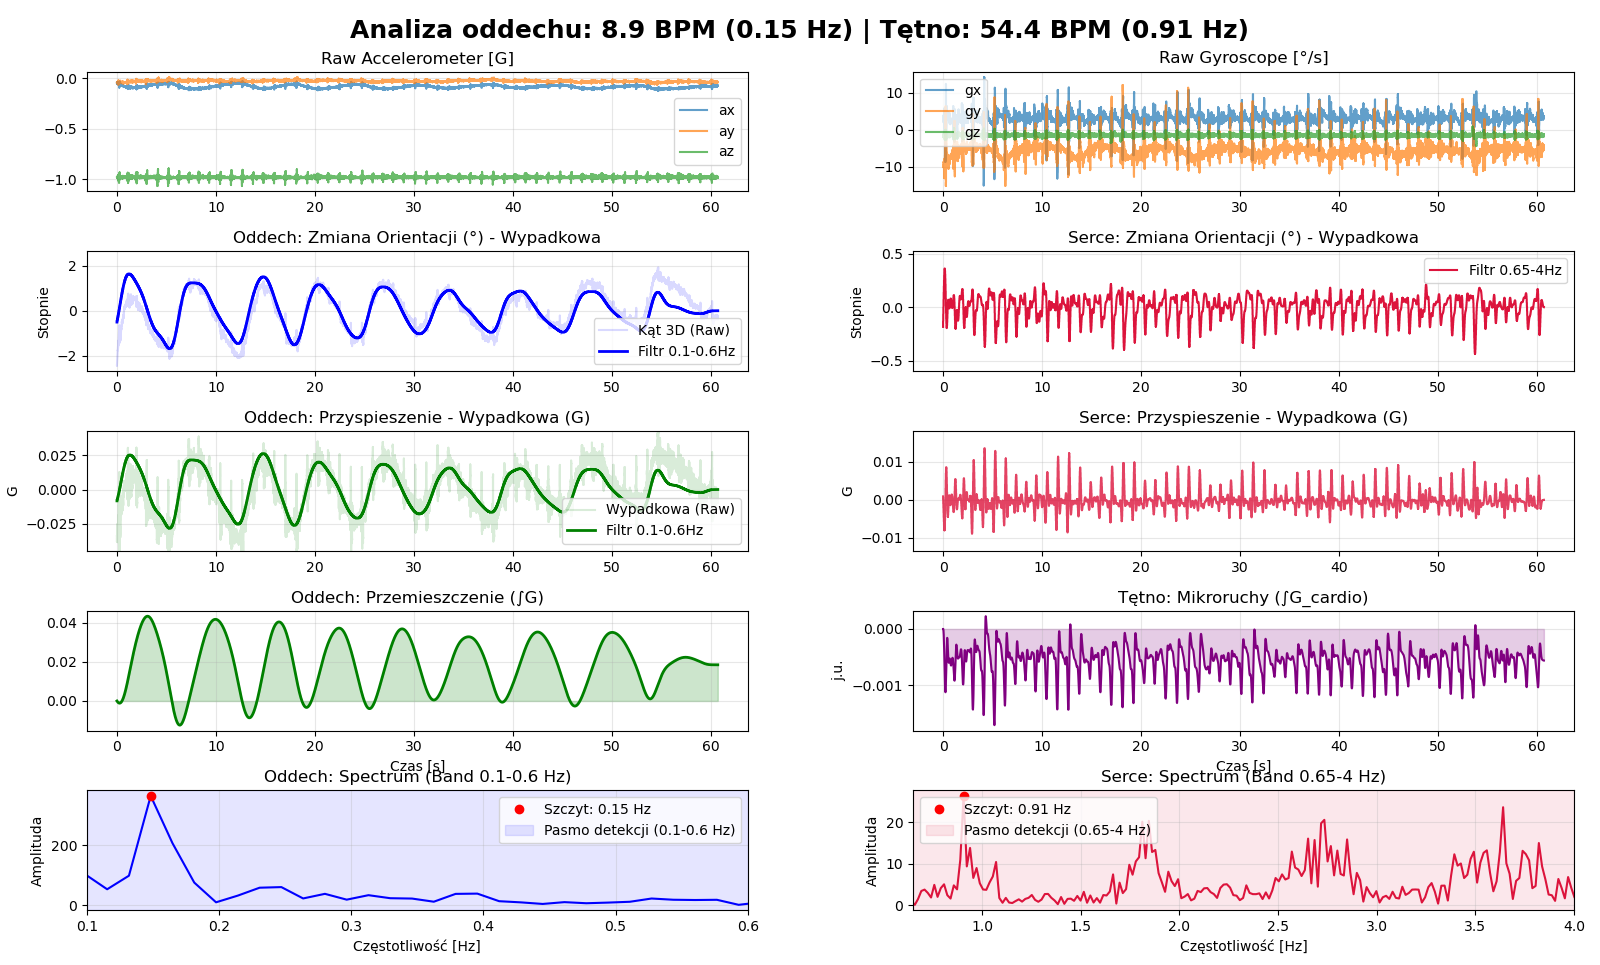
\includegraphics[height=0.72\textheight,keepaspectratio]{plots_imu/acc.png}
        \caption{Zestawienie 10 wykresów analizy sygnału z modułu LSM6DS3: dane surowe, sygnał oddechowy oraz analiza tętna.}
    \end{figure}
\end{frame}

\begin{frame}{Stanowisko pomiarowe -- IMU}
    \begin{figure}
        \centering
        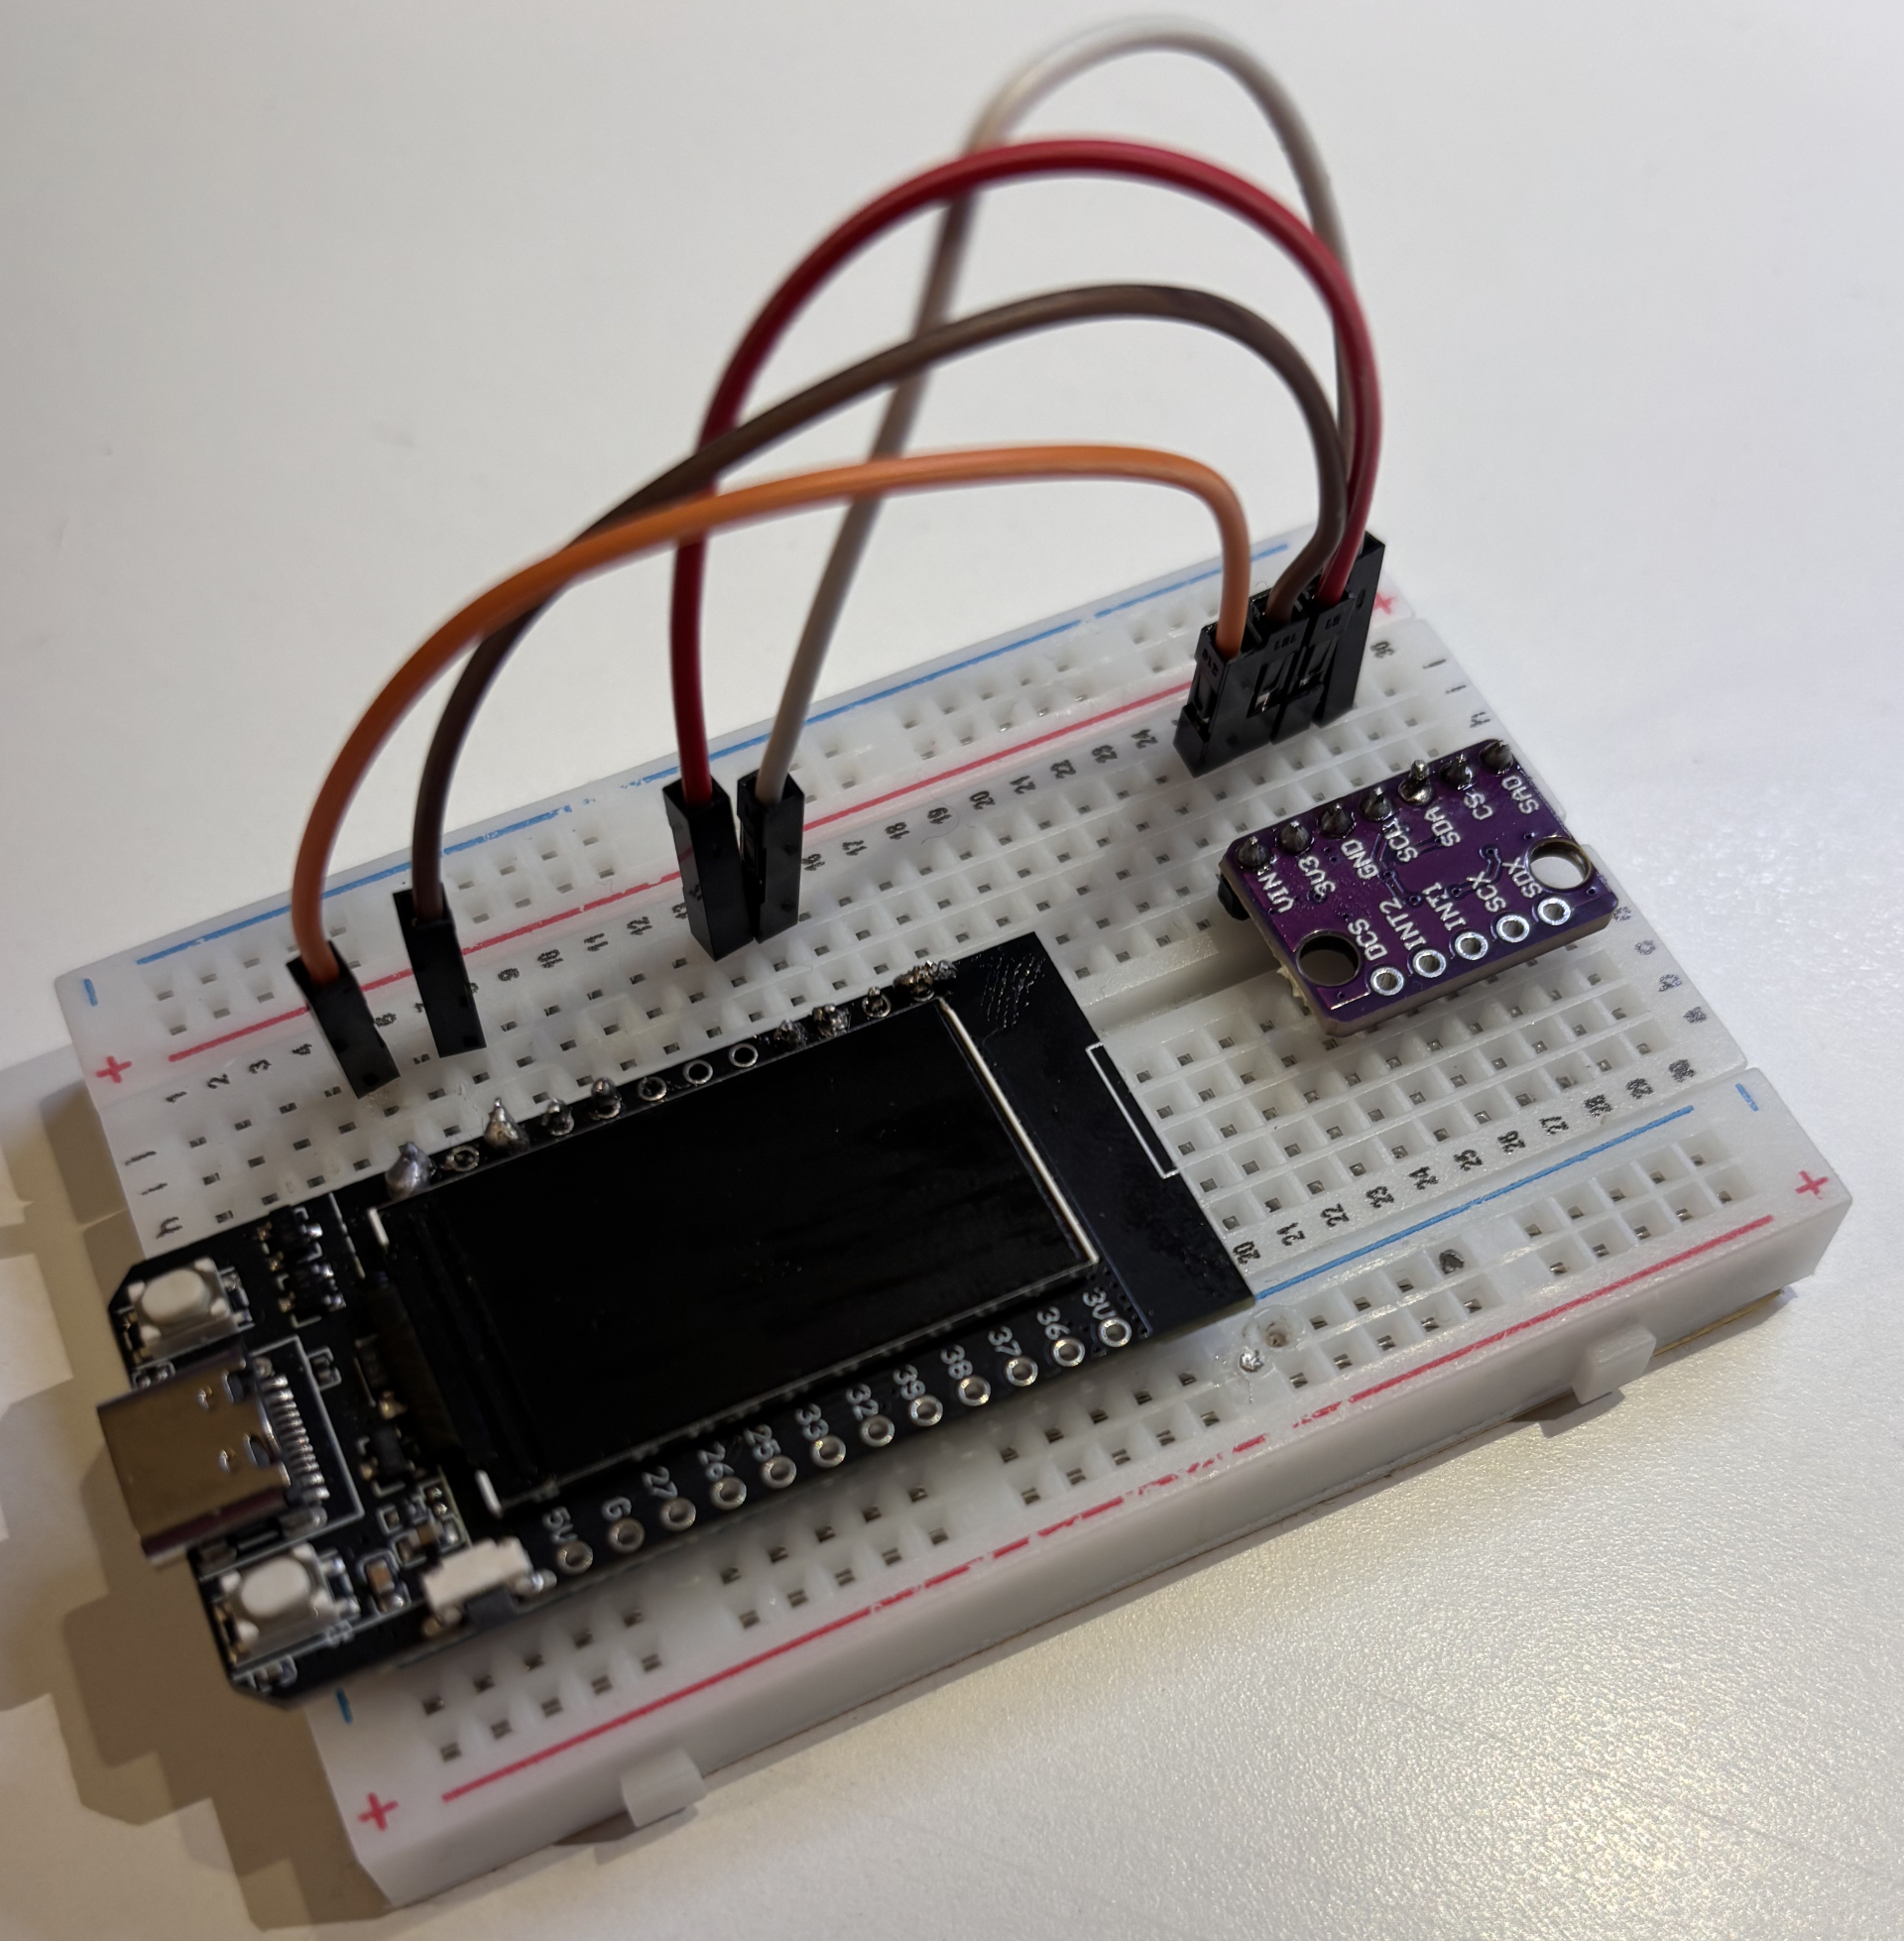
\includegraphics[width=0.75\textwidth,keepaspectratio]{plots_imu/imu_.png}
        \caption{Moduł IMU LSM6DS3 połączony z mikrokontrolerem ESP32.}
    \end{figure}
\end{frame}

\begin{frame}{Aktualny stan pracy -- Radar Dopplerowski (HB100)}
    \begin{itemize}
        \item \textbf{Akwizycja i Hardware:} 
        \begin{itemize}
            \item Przetestowano tani moduł mikrofalowy (HB100).
            \item Główny problem: bardzo niska amplituda sygnału wyjściowego ($\sim$5 mV).
            \item Rozwiązanie: Zaprojektowano i zbudowano dedykowany układ filtru i wzmacniacza na układzie MCP6002.
        \end{itemize}
        \item \textbf{Wyniki i analiza (zmiany napięcia):}
        \begin{itemize}
            \item Wyraźny sygnał oddechu z odległości ok. 60 cm od klatki piersiowej.
            \item Wstrzymanie oddechu odsłania oscylacje odpowiadające pracy serca (tętno jest detekowalne).
        \end{itemize}
        \item \textbf{Oprogramowanie:} Stworzono moduł w Pythonie (\texttt{radar\_viewer.py}) z szybkim odczytem (921600 baud) z ESP32 do analizy i rysowania wykresów FFT na żywo.
    \end{itemize}
\end{frame}

\begin{frame}{Analiza Radarowa -- Widmo sygnału}
    \begin{figure}
        \centering
        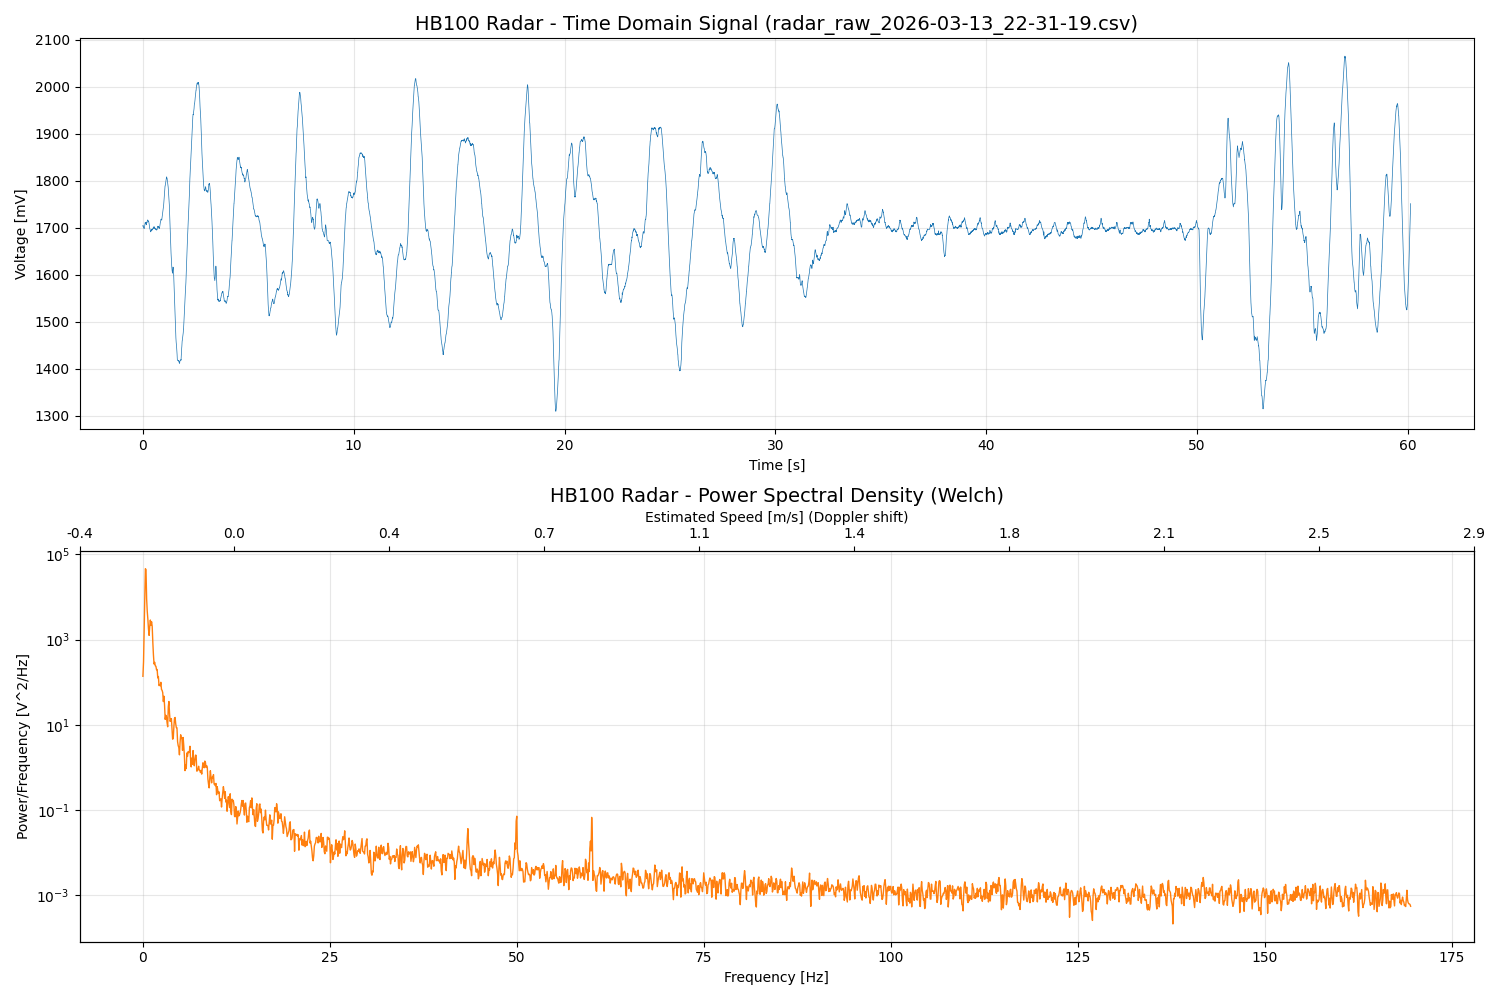
\includegraphics[width=0.9\textwidth,keepaspectratio]{plots_radar/radar_raw_2026-03-13_22-31-19.png}
        \caption{Zapis surowego sygnału radaru HB100 wraz z analizą gęstości widmowej mocy (metoda Welcha), pozwalającą na estymację prędkości z przesunięcia Dopplera.}
    \end{figure}
\end{frame}

\begin{frame}{Stanowisko pomiarowe -- Radar HB100}
    \begin{columns}
        \column{0.5\textwidth}
        \centering
        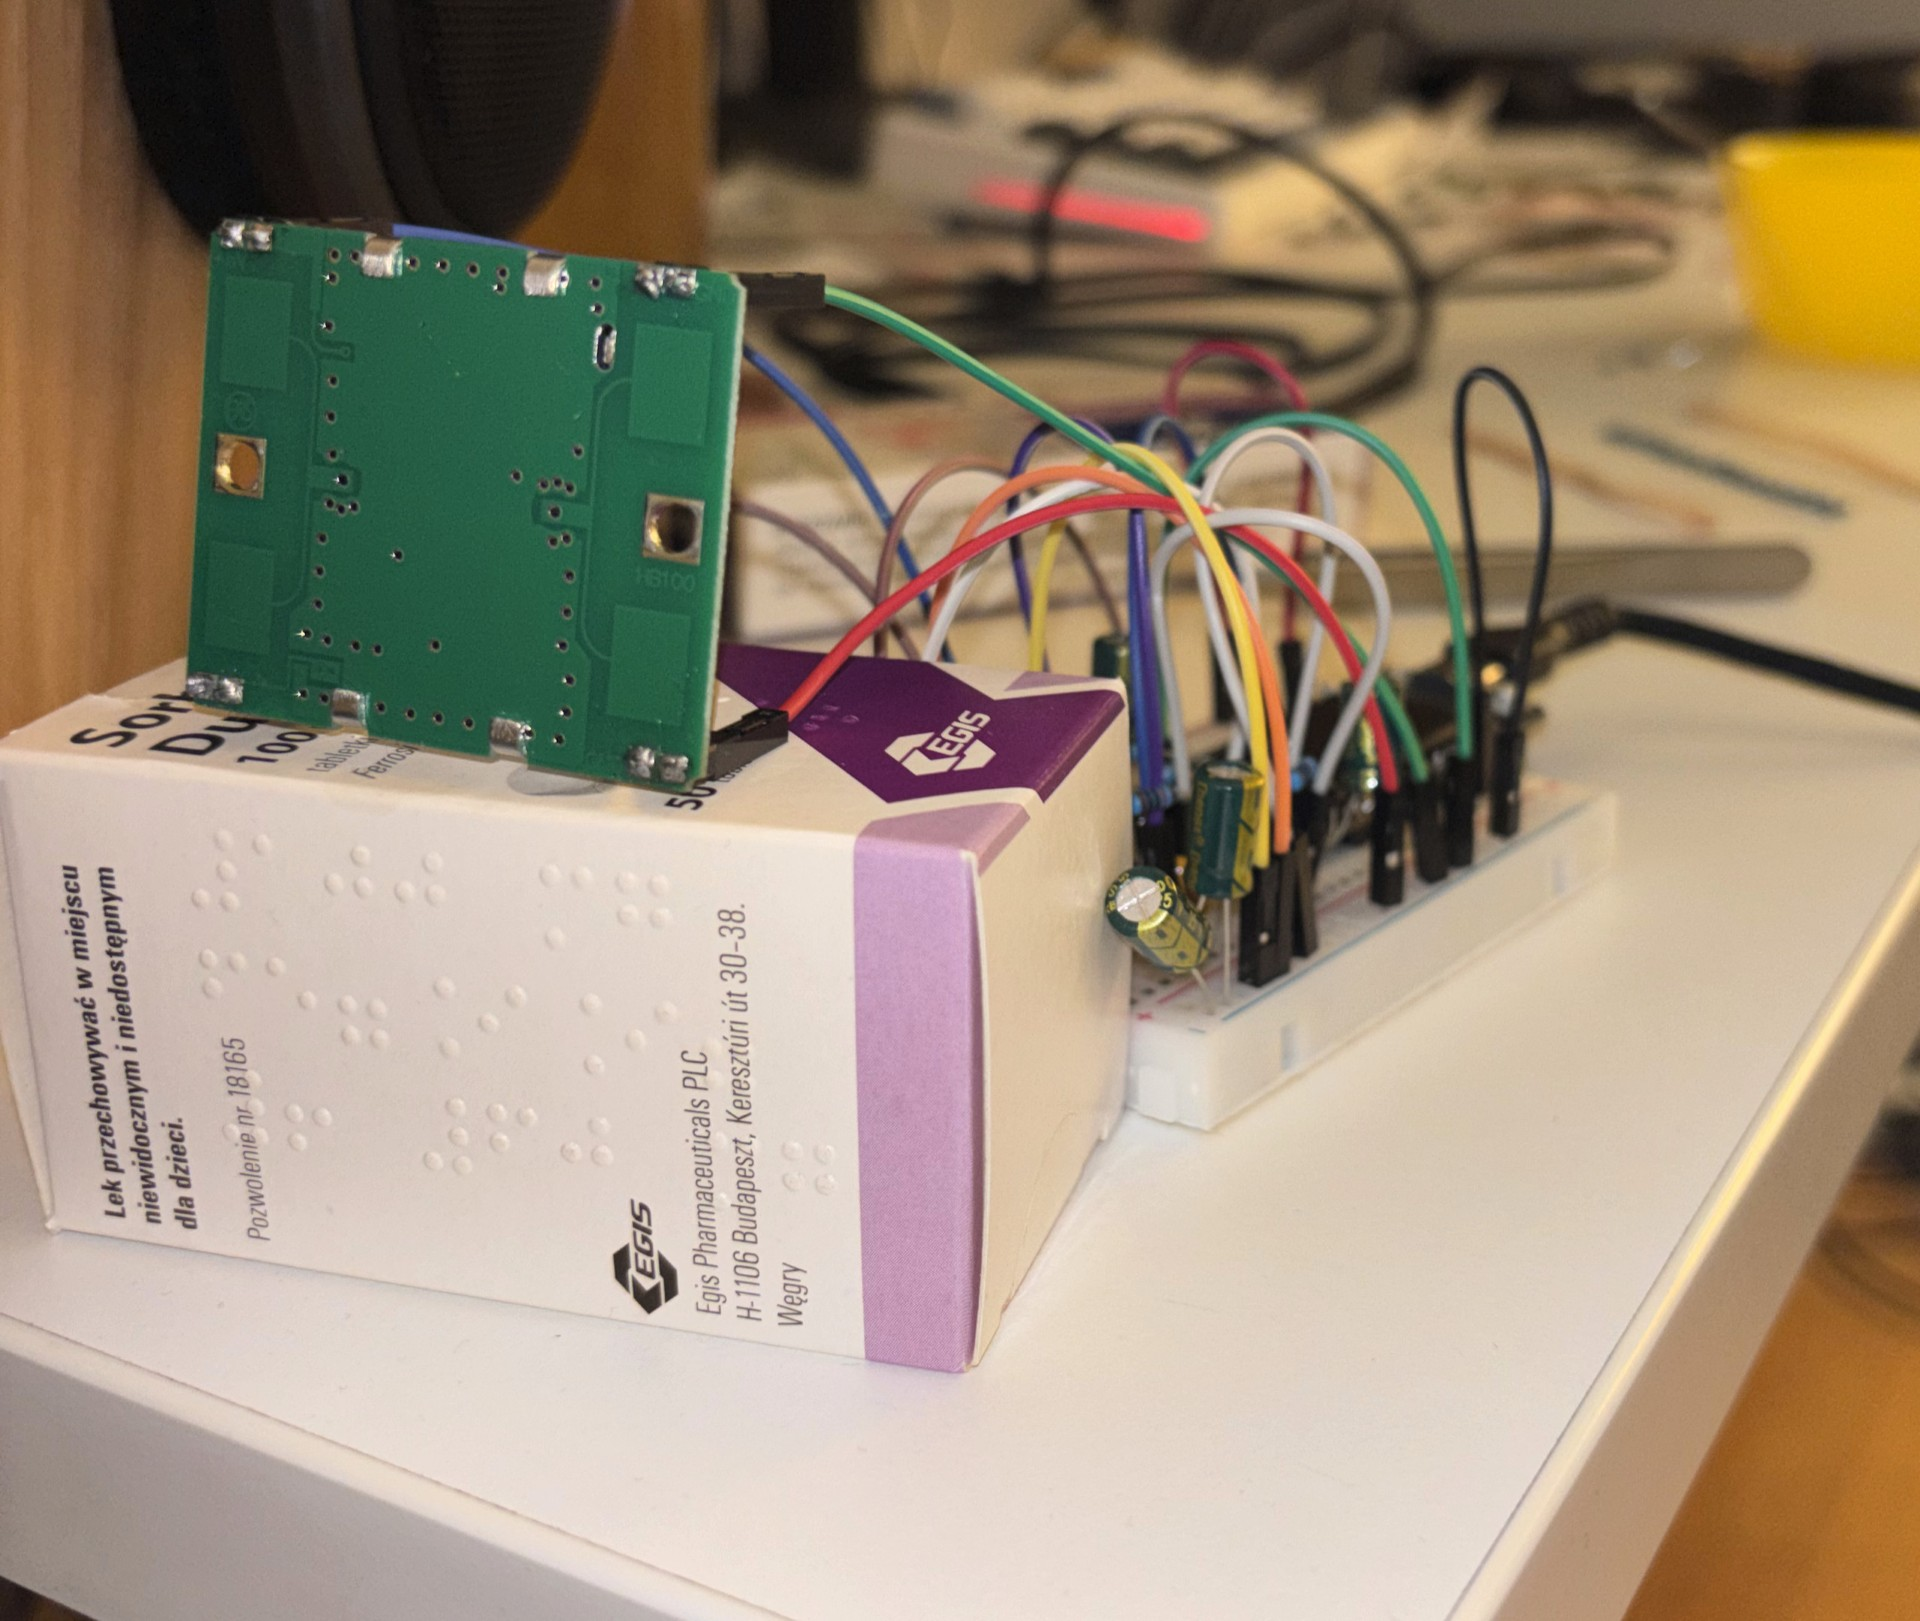
\includegraphics[width=\textwidth,keepaspectratio]{plots_radar/radar_.jpg}
        \column{0.5\textwidth}
        \centering
        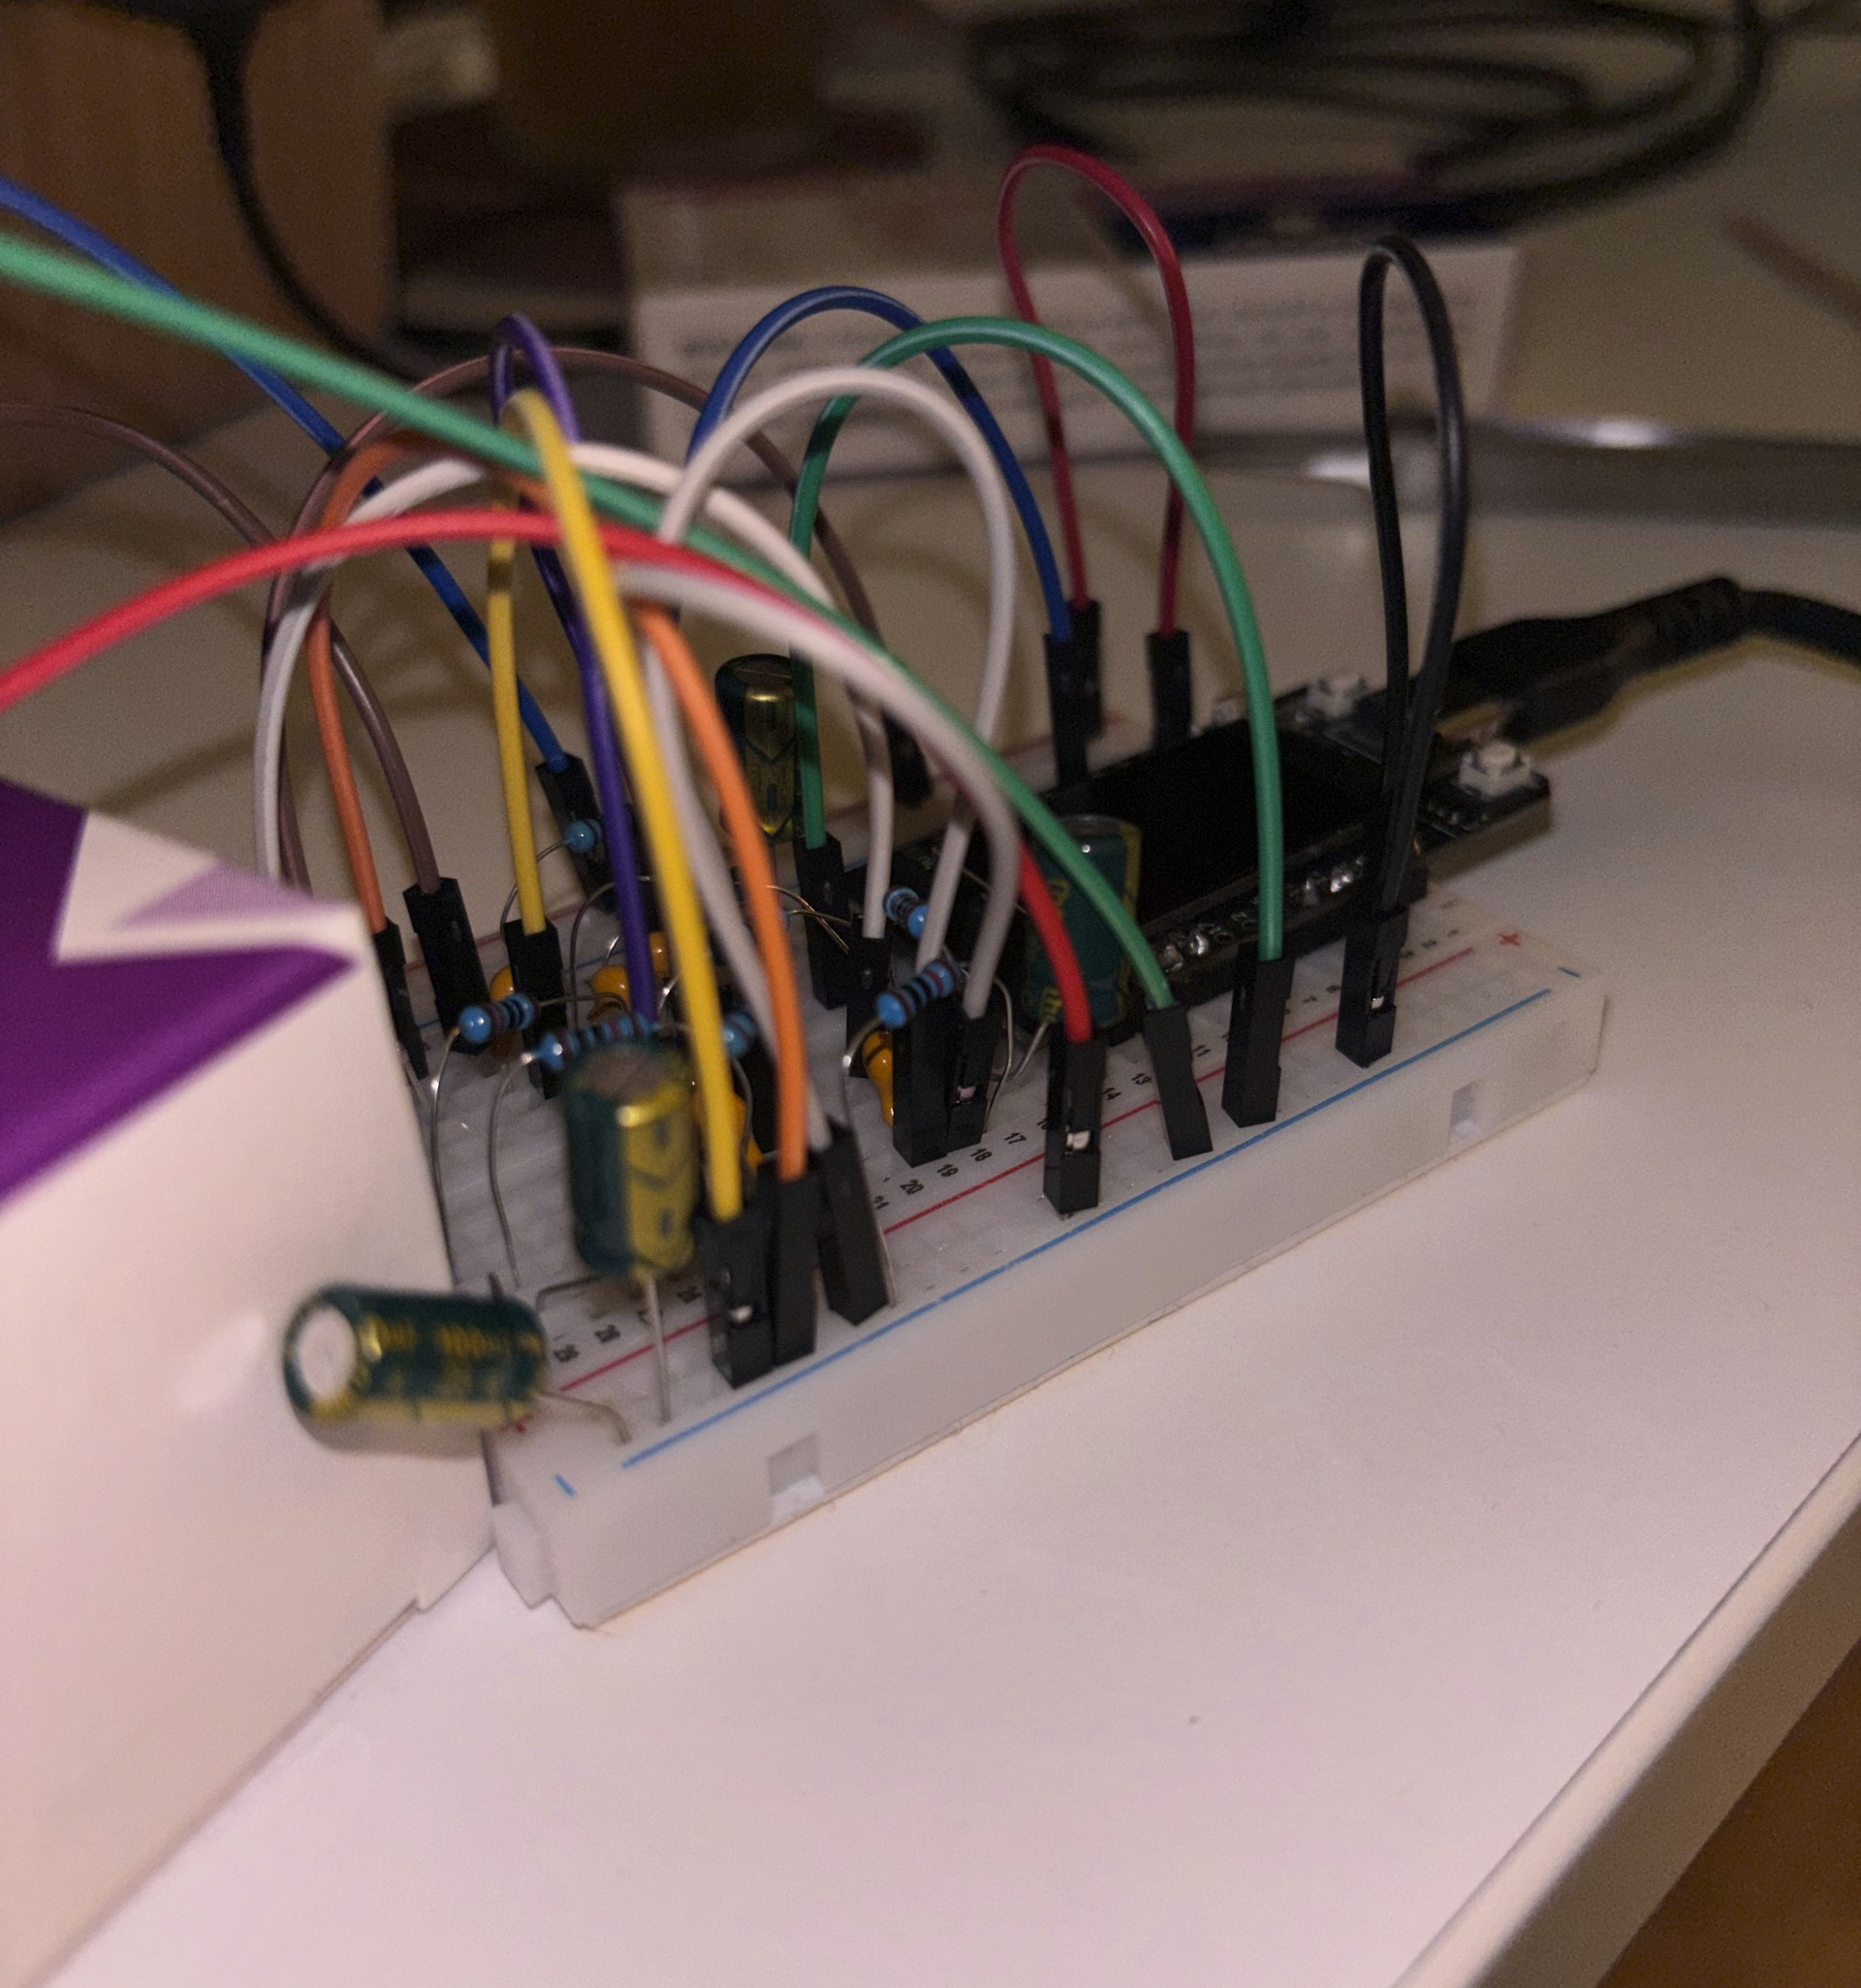
\includegraphics[width=\textwidth,keepaspectratio]{plots_radar/radar_2.jpg}
    \end{columns}
    \vspace{0.3cm}
    \centering
    \small Zdjęcia poglądowe modułu radaru HB100 oraz stanowiska testowego.
\end{frame}

\begin{frame}{Harmonogram prac -- Najbliższe kroki}
    \textbf{Faza testów i ulepszanie torów pomiarowych (Do 20 Czerwca 2026):}
    \begin{itemize}
        \item Przetestowanie sygnału IMU i porównanie go z danymi bezpośrednio z telefonu komórkowego.
        \item Rozszerzone testy radaru HB100 (różne warianty montażu, folia aluminiowa na klatce piersiowej do wzmocnienia odbicia).
        \item Uruchomienie precyzyjnego radaru \textbf{Acconeer A121} (bazującego na bezpośrednich zmianach fazy).
    \end{itemize}
    \textbf{Zakończenie testów i sieci neuronowe (Wrzesień -- Październik 2026):}
    \begin{itemize}
        \item Zebranie finalnej, obszernej bazy danych i klasyfikacja sygnałów.
        \item Implementacja i ewaluacja modeli uczenia maszynowego.
    \end{itemize}
    \textbf{Redakcja tekstu pracy inżynierskiej (Listopad 2026):}
    \begin{itemize}
        \item Kompletowanie części literaturowej, podsumowanie wyników, redakcja ostatecznej wersji pracy.
    \end{itemize}
\end{frame}

\begin{frame}{Podsumowanie}
    \begin{itemize}
        \item Prace implementacyjne postępują zgodnie z założeniami.
        \item Opracowano poprawnie działające środowiska testowe zarówno dla czujników inercyjnych, jak i radaru analogowego.
        \item Zbudowano wymagane układy elektroniczne i rozwiązano wstępne problemy z poziomem sygnałów.
        \item Główne wyzwania na kolejne miesiące to integracja lepszego modułu radarowego, przygotowanie bazy danych oraz faza trenowania sztucznej inteligencji.
    \end{itemize}
    
    \vspace{1cm}
    \begin{center}
        \Large Dziękuję za uwagę!
    \end{center}
\end{frame}

\end{document}
